\NeedsTeXFormat{LaTeX2e}
%\PassOptionsToClass{handout}{beamer}
\documentclass{beamer}
\usepackage{beamerPack}
\usepackage[boxed,ruled,vlined]{algorithm2e}
\usepackage{setspace}
\usepackage[usestackEOL]{stackengine}[2013-10-15]
\def\x{\hspace{4.1ex}}    %BETWEEN TWO 1-DIGIT NUMBERS
\def\y{\hspace{3.4ex}}  %BETWEEN 1 AND 2 DIGIT NUMBERS
\def\z{\hspace{2.7ex}}    %BETWEEN TWO 2-DIGIT NUMBERS
\usepackage[04]{../lecture}
\subtitle{}
\begin{document}

\begin{frame}[fragile]{}
\titlepage
\end{frame}

\section{algorithm design}		%%%%%%%%
\subsection{}

\begin{frame}[fragile]{問題解決の枠組み}{}
\begin{align*}
アルゴリズム =& 前処理? \\
&+ 相似問題^{+} \\
&+ 後処理?
\end{align*}

記号は正規表現より輸入

\begin{codeof}{language=Rust}{skeleton}
fn solve(problem) {
  // pre-process
  ...
  solve(sub-problem1);
  solve(sub-problem2);
  // post-process
  ...
  return;
\end{codeof}
\end{frame}

\begin{frame}[fragile]{例1}{Fibonacchi}

\begin{align*}
Fib(1) =& 1 \\
Fib(2) =& 1 \\
Fib(n) =& Fib(n - 1) + Fix(n -2) \quad (3 \le n)\\
\end{align*}
\end{frame}

\begin{frame}[fragile]{例2}{Ackermann and Takeuchi}
\begin{align*}
A(0, n) =& n + 1 \\
A(m, 0) =& A(m - 1, 1) \\
A(m, n) =& A(m - 1, A(m, n - 1))
\end{align*}

\begin{align*}
Tak(x, y, z) =& y if x \le y \\
=& Tak(Tak(x - 1, y, z), Tak(y -1, z, x), Tak(z - 1, x, y))
\end{align*}

線形再帰ならループと再帰の記述の手間は同じ(実行時間も同じ)。
問題は線形でない場合:スタックを使って自分で機械語実行過程のシミュレーションを書けるならOK。
\end{frame}

\begin{frame}[fragile]{文章題1:Pascalの三角形}{}
\stackMath
\Longstack[l]{
n=0\\
n=1\\
n=2\\
n=3\\
n=4\\
n=5\\
n=6\qquad\ \\
}
\Longstack{
1\\
1\x 1\\
1\x 2\x 1\\
1\x 3\x 3\x 1\\
1\x 4\x 6\x 4\x 1\\
1\x 5\y 10\z 10\y 5\x 1\\
1\x 6\y 15\z 20\z 15\y 6\x 1\\
1\x 7\x 21\z 35\z 35\z 21\y 7\x 1\\
}

$n = 23$, 左から11番目の数は?
\end{frame}

\begin{frame}[fragile]{Pascalの三角形}{北東+北西に等しい}

\begin{align*}
P(n,k) &= P(n-1, k - 1) + P(n - 1, k)
\end{align*}

\begin{center}
\rotatebox{-45}{
\scalebox{0.6}{
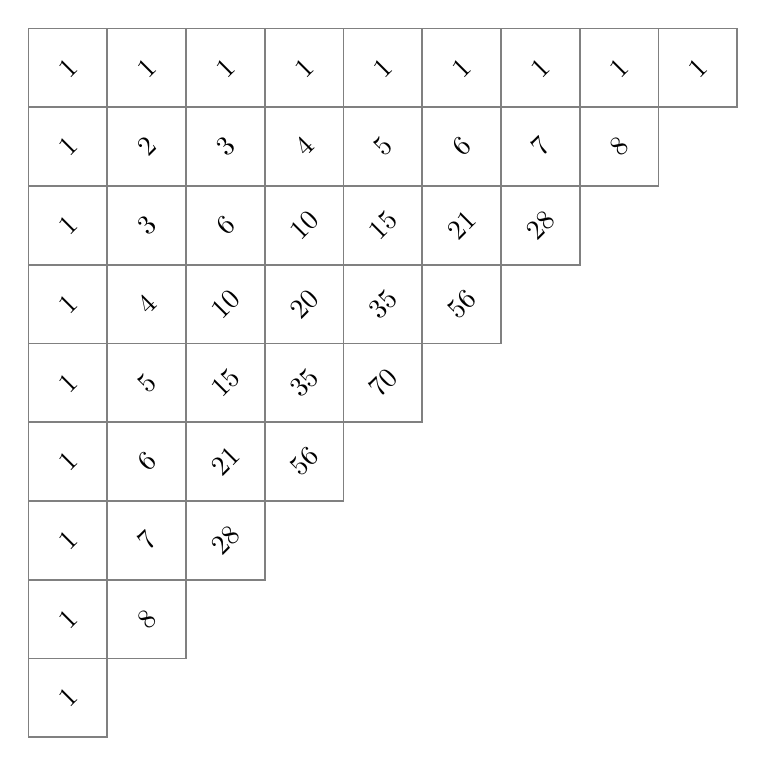
\begin{tikzpicture}[cell/.style = {rectangle,draw=gray,semithick,minimum size=1cm,outer sep=0mm}]
\foreach \i [count=\j from 0] in {1, 1, 1, 1, 1,  1, 1, 1, 1}
    \node[cell] at (\j,  0) {\rotatebox{45}{$\i$}};
\foreach \i [count=\j from 0] in {1, 2, 3, 4, 5,  6, 7, 8}
    \node[cell] at (\j, -1) {\rotatebox{45}{$\i$}};
\foreach \i [count=\j from 0] in {1, 3, 6, 10,15,21,28}
    \node[cell] at (\j, -2) {\rotatebox{45}{$\i$}};
\foreach \i [count=\j from 0] in {1, 4, 10,20,35,56}
    \node[cell] at (\j, -3) {\rotatebox{45}{$\i$}};
\foreach \i [count=\j from 0] in {1, 5, 15,35,70}
    \node[cell] at (\j, -4) {\rotatebox{45}{$\i$}};
\foreach \i [count=\j from 0] in {1, 6, 21,56}
    \node[cell] at (\j, -5) {\rotatebox{45}{$\i$}};
\foreach \i [count=\j from 0] in {1, 7, 28}
    \node[cell] at (\j, -6) {\rotatebox{45}{$\i$}};
\foreach \i [count=\j from 0] in {1, 8}
    \node[cell] at (\j, -7) {\rotatebox{45}{$\i$}};
\foreach \i [count=\j from 0] in {1}
    \node[cell] at (\j, -8) {\rotatebox{45}{$\i$}};
\end{tikzpicture}
}
}
\end{center}
\end{frame}

\begin{frame}[fragile]{飛行経路の総数を求めよ}{}
観光用スペースシャトルが高度100キロメートルからツアーを開始します。乗客は1分ごとに次の1分間上昇するか、下降するかを決めることができます。どちらも1分でちょうど1キロ上昇するか下降します。11分後に元の高度に戻ってこなければならないとすると、飛行経路は何通りあるでしょう。
\end{frame}

\begin{frame}[fragile]{}{}
\begin{center}
\rotatebox{45}{
\scalebox{0.5}{
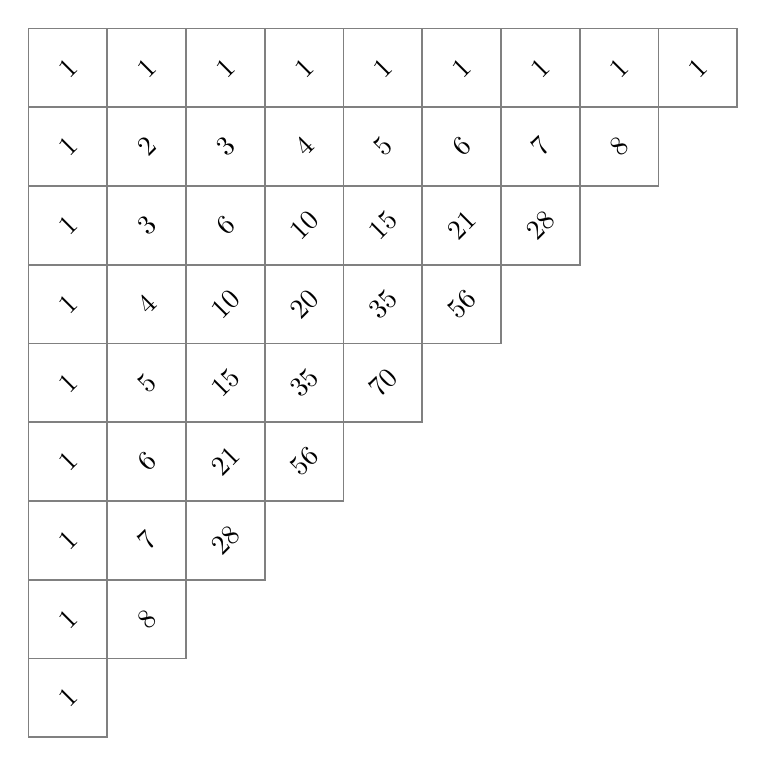
\begin{tikzpicture}[cell/.style = {rectangle,draw=gray,semithick,minimum size=1cm,outer sep=0mm}]
\foreach \i [count=\j from 0] in {1, 1, 1, 1, 1,  1, 1, 1, 1}
    \node[cell] at (\j,  0) {\rotatebox{45}{$\i$}};
\foreach \i [count=\j from 0] in {1, 2, 3, 4, 5,  6, 7, 8}
    \node[cell] at (\j, -1) {\rotatebox{45}{$\i$}};
\foreach \i [count=\j from 0] in {1, 3, 6, 10,15,21,28}
    \node[cell] at (\j, -2) {\rotatebox{45}{$\i$}};
\foreach \i [count=\j from 0] in {1, 4, 10,20,35,56}
    \node[cell] at (\j, -3) {\rotatebox{45}{$\i$}};
\foreach \i [count=\j from 0] in {1, 5, 15,35,70}
    \node[cell] at (\j, -4) {\rotatebox{45}{$\i$}};
\foreach \i [count=\j from 0] in {1, 6, 21,56}
    \node[cell] at (\j, -5) {\rotatebox{45}{$\i$}};
\foreach \i [count=\j from 0] in {1, 7, 28}
    \node[cell] at (\j, -6) {\rotatebox{45}{$\i$}};
\foreach \i [count=\j from 0] in {1, 8}
    \node[cell] at (\j, -7) {\rotatebox{45}{$\i$}};
\foreach \i [count=\j from 0] in {1}
    \node[cell] at (\j, -8) {\rotatebox{45}{$\i$}};
\end{tikzpicture}
}
}
\end{center}
\end{frame}

\begin{frame}[fragile]{飛行経路の総数を求めよ}{}
観光用飛行機が高度5キロメートルからツアーを開始します。乗客は1分ごとに次の1分間上昇するか、下降するかを決めることができます。どちらも1分でちょうど1キロ上昇するか下降します。11分後に元の高度に戻ってこなければならないとすると、飛行経路は何通りあるでしょう。高度0キロメートルで墜落します。
\end{frame}

\begin{frame}[fragile]{}{}
\begin{center}
\rotatebox{45}{
\scalebox{0.5}{
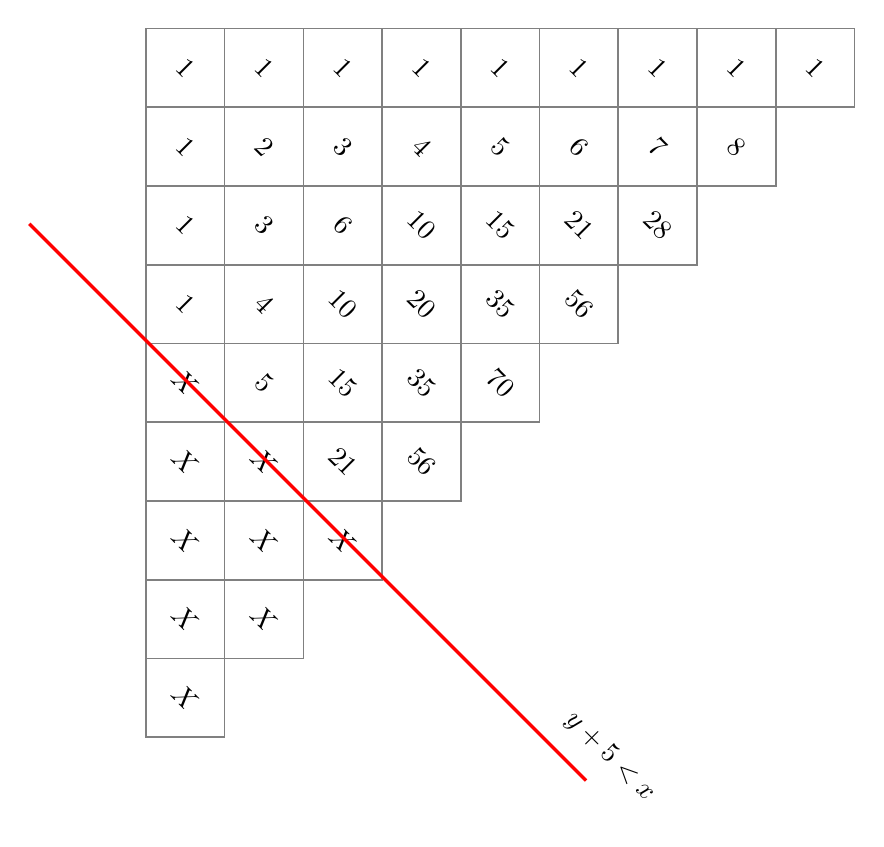
\begin{tikzpicture}[cell/.style = {rectangle,draw=gray,semithick,minimum size=1cm,outer sep=0mm}]
\foreach \i [count=\j from 0] in {1, 1, 1, 1, 1, 1, 1, 1, 1}
    \node[cell] at (\j,  0) {\rotatebox{-45}{$\i$}};
\foreach \i [count=\j from 0] in {1, 2, 3, 4, 5,  6, 7, 8}
    \node[cell] at (\j, -1) {\rotatebox{-45}{$\i$}};
\foreach \i [count=\j from 0] in {1, 3, 6, 10,15,21,28}
    \node[cell] at (\j, -2) {\rotatebox{-45}{$\i$}};
\foreach \i [count=\j from 0] in {1, 4, 10,20,35,56}
    \node[cell] at (\j, -3) {\rotatebox{-45}{$\i$}};
\foreach \i [count=\j from 0] in {X, 5, 15, 35, 70}
    \node[cell] at (\j, -4) {\rotatebox{-45}{$\i$}};
\foreach \i [count=\j from 0] in {X, X, 21, 56}
    \node[cell] at (\j, -5) {\rotatebox{-45}{$\i$}};
\foreach \i [count=\j from 0] in {X, X, X}
    \node[cell] at (\j, -6) {\rotatebox{-45}{$\i$}};
\foreach \i [count=\j from 0] in {X, X}
    \node[cell] at (\j, -7) {\rotatebox{-45}{$\i$}};
\foreach \i [count=\j from 0] in {X}
    \node[cell] at (\j, -8) {\rotatebox{-45}{$\i$}};
\draw[draw=red,rotate=-45,very thick] (0,-2.8) --  ++(10,0) node[rotate=-45,above=4pt] () {$y + 5 < x$};
\end{tikzpicture}
}
}
\end{center}
\end{frame}

\begin{frame}[fragile]{素朴なアルゴリズムと巧妙なアルゴリズムの違い}{}
\begin{itemize}%\itemsep8pt
\item 時間計算量を減らす:無駄を省く
\item 空間計算量を減らす:無駄を省く
\end{itemize}

\vfill
空間計算量を減らす例は前回出てきたpartition。元々は一つの配列から二つの配列に要素をコピー(移動)させるアルゴリズムだったが、効率を追求した結果、あのようなプログラム定義になった。
\end{frame}

\begin{frame}[fragile]{素数の計算}{}
この話は相似問題に等価なものが含まれるので削除する話なので、今回の最後か次回がふさわしい。
\end{frame}

\section{for programmers}		%%%%%%%%
\subsection{}

\begin{frame}[fragile]{数学的解析の力}{}

\[
Fib(n) = \frac{1}{\sqrt{5}}
\left\{
\left(\frac{1 + \sqrt{5}}{2}\right)^n
-
\left(\frac{1 - \sqrt{5}}{2}\right)^n
\right\}
\]

\end{frame}

\begin{frame}[fragile]{ふかしぎおねえさん}{}
a
\end{frame}

\end{document}
